\documentclass[problem]{mcs}

\begin{pcomments}
  \pcomment{FP_directed_graphs_and_probability} %\pcomment{from: S09.cp7r}
  \pcomment{prepared in Fall'11 for the final exam by S. Dwivedi & ARM}
  \pcomment{ARM edited 12/20/11}
\end{pcomments}

\pkeywords{
  digraphs
  DAGs
  probability
}

%%%%%%%%%%%%%%%%%%%%%%%%%%%%%%%%%%%%%%%%%%%%%%%%%%%%%%%%%%%%%%%%%%%%%
% Problem starts here
%%%%%%%%%%%%%%%%%%%%%%%%%%%%%%%%%%%%%%%%%%%%%%%%%%%%%%%%%%%%%%%%%%%%%

\newcommand{\Gdir}{\overrightarrow{G}}

\begin{problem}
\bparts

\ppart For the directed acyclic graph (DAG) $G_0$ in
Figure~\ref{fig:Gdir}, a minimum-edge DAG with the same walk relation
can be obtained by removing some edges.  List these edges (use
notation $\diredge{u}{v}$ for an edge from $u$ to $v$):

\exambox{1.5in}{0.5in}{-0.5in}

\begin{figure}
\begin{center}
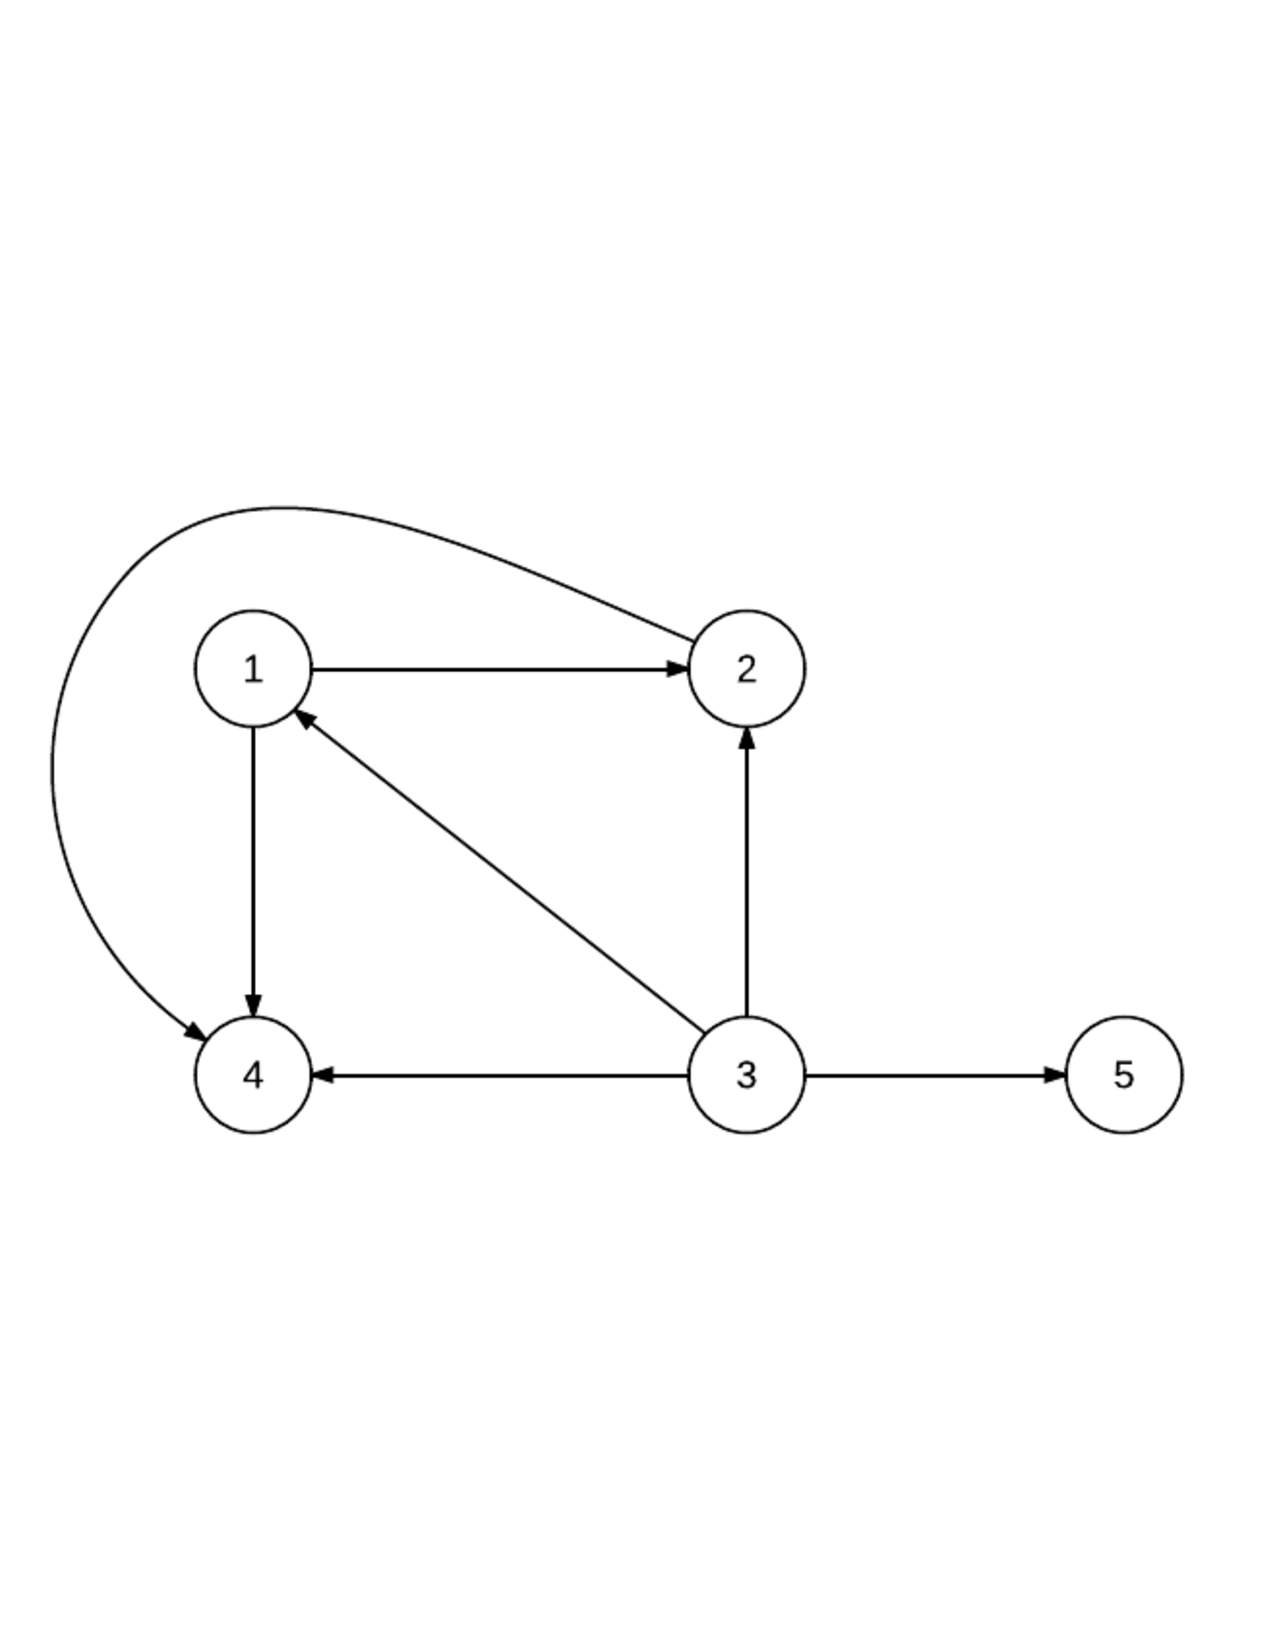
\includegraphics[width = 3.0in, height = 3.5in]{dir_graph}
\end{center}
\caption{The DAG $G_0$}
\label{fig:Gdir}
\end{figure}

\begin{solution}
After removing edges $\diredge{1}{4}$, $\diredge{3}{2}$ and
$\diredge{3}{4}$, we get the minimum DAG.
\end{solution}

\ppart List the vertices in a maximal chain in $G_0$.

\exambox{1.5in}{0.5in}{-0.3in}

\begin{solution}
$\set{3,1,2,4}$
\end{solution}
\eparts

\vspace{0.3in}
Let $G$ be the simple graph shown in Figure ~\ref{fig:simpleG}.

\begin{figure}
\begin{center}
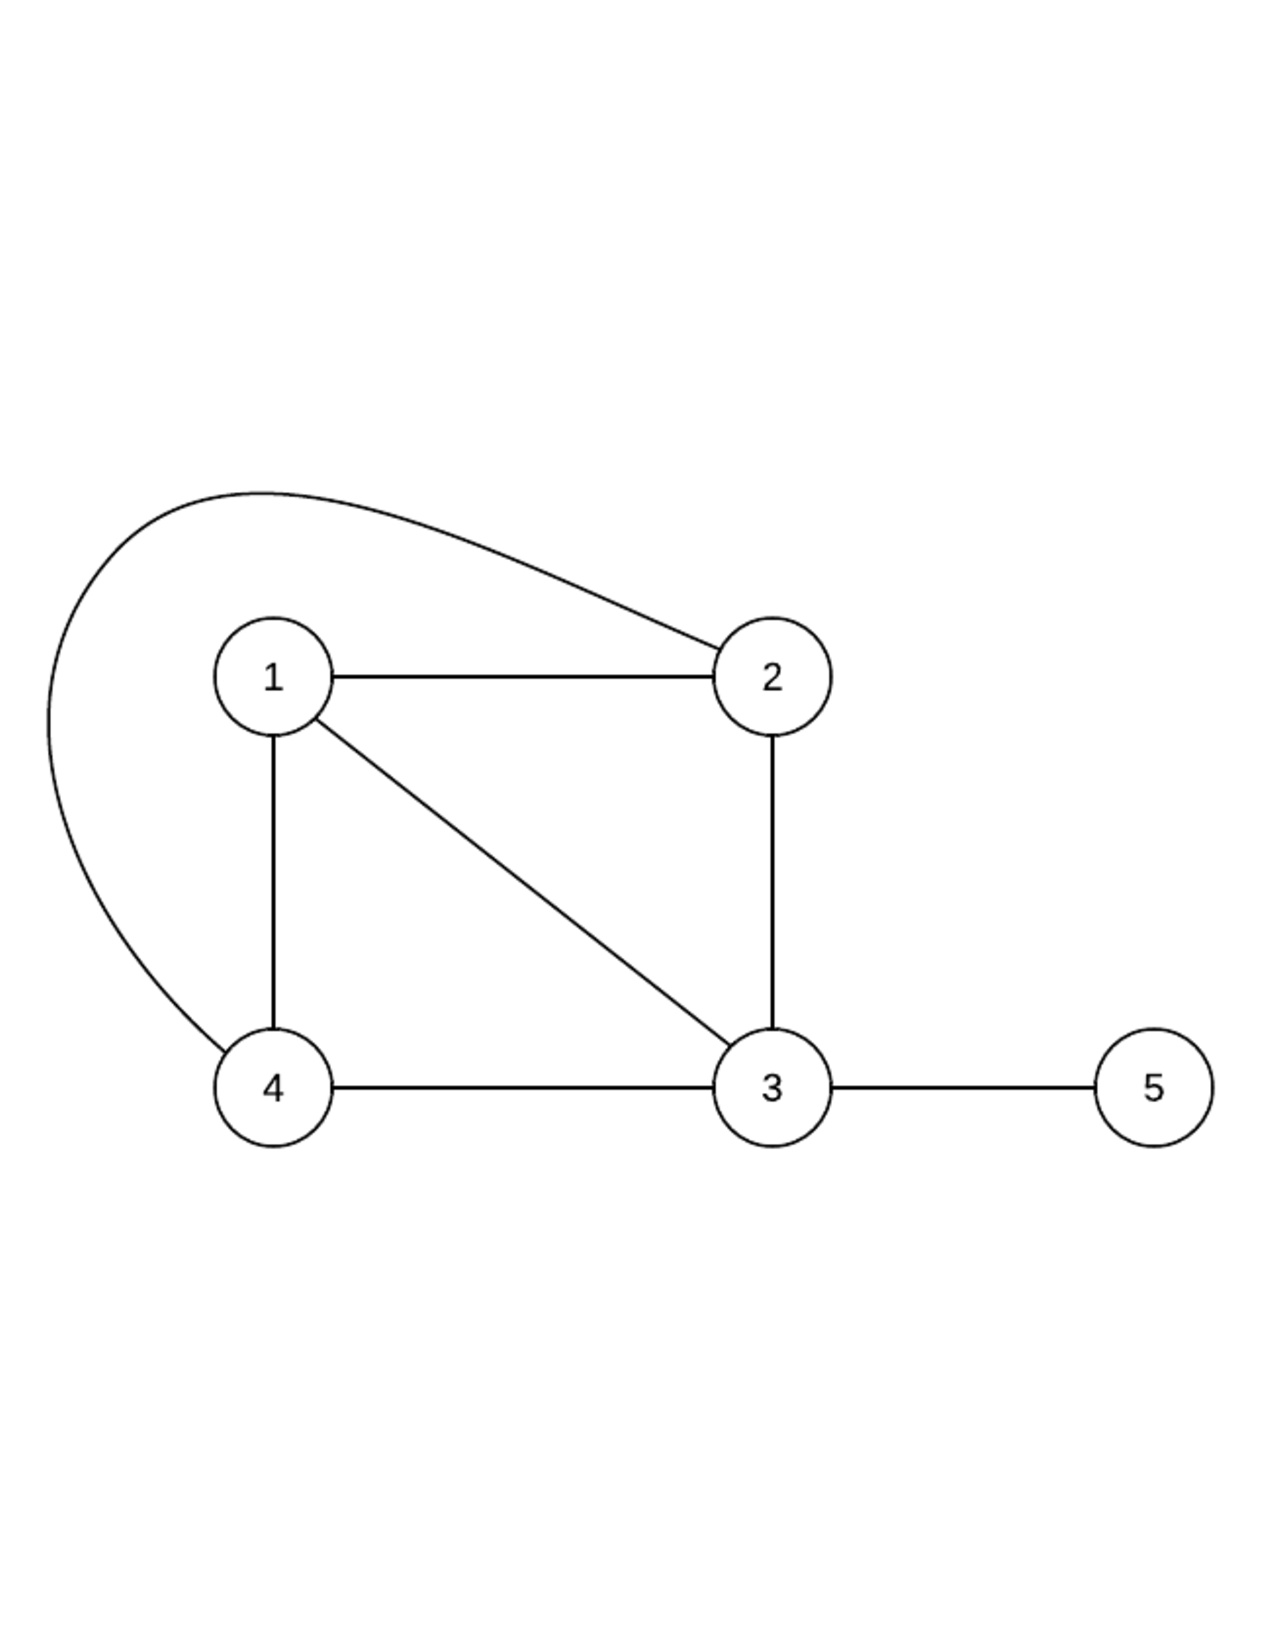
\includegraphics[width = 3.0in, height = 3.5in]{simple_graph} 
%\includegraphics[width=6in,height=7in]{mq1.jpg}
\end{center}
\caption{Simple graph $G$}
\label{fig:simpleG}
\end{figure}

A directed graph $\Gdir$ can be randomly constructed from
$G$ by assigning a direction to each edge independently with
equal likelihood.

\bparts

\ppart What is the probability that $\Gdir = G_0$?

\exambox{0.5in}{0.5in}{-0.3in}


\begin{solution}
\[
2^{-\card{\edges{G}}} = 2^{-7} =\frac{1}{128}
\]
\end{solution}

\eparts

\examspace

Define the following events with respect to the random graph
$\Gdir$:
\begin{align*}
T_1 & \eqdef \text{vertices } 2,3,4 \text{ are on a length three directed cycle},\\
T_2 & \eqdef \text{vertices } 1,3,4 \text{ are on a length three directed cycle},\\
T_3 & \eqdef \text{vertices } 1,2,4 \text{ are on a length three directed cycle},\\
T_4 & \eqdef \text{vertices } 1,2,3 \text{ are on a length three directed cycle}.
\end{align*}

\bparts

\ppart\label{prT1T1T2} What is
\begin{align*}
\pr{T_1}?                               & \examrule[0.75in]\\
\\
\pr{T_1 \intersect T_2}?                & \examrule[0.75in]\\
\\
\pr{T_1 \intersect T_2 \intersect T_3}? & \examrule[0.75in]
\end{align*}
\examspace[1in]

\begin{solution}
\begin{align*}
\pr{T_1} = \frac{2}{2^3} & = \frac{1}{4}\\
\pr{T_1 \intersect T_2}  & = \frac{1}{16}\\
\pr{T_1 \intersect T_2 \intersect T_3}
                        & = 0.
\end{align*}
\end{solution}

\examspace

\ppart $\Gdir$ has the property that if it has a directed cycle, then
it has a length three directed cycle.  Use this fact to find the
probability that $\Gdir$ is a DAG.

\exambox{2.5in}{0.5in}{-0.8in}

%\examspace[3in]

\begin{solution}
The only possible length three directed cycles are the ones described by
$T_1,\dots,T_4$.  So the given property implies that $\Gdir$ is a DAG
iff $\lgunion_{i \in \Zintv{1}{4}} T_i$ does \emph{not} occur.

Now using the Inclusion-Exclusion principle,

\begin{align*}
\pr{\Gdir \text{ is a DAG}}
   & = 1 - \pr{T_1 \union T_2 \union T_3 \union T_4}\\
   & = 1 - \sum_{i \in \Zintv{1}{4}} \pr{T_i} + \sum_{i\neq j} \pr{T_i \intersect T_j}\\
   & \quad - \sum_{i\neq j \neq k} \pr{T_i \intersect T_j \intersect T_k}
        + \pr{T_1 \intersect T_2 \intersect T_3 \intersect T_4}\\
   & = 1 - 4 \cdot \frac{1}{4} + 6 \cdot \frac{1}{16} - 0 + 0\\
   & = \frac{3}{8}
\end{align*}
Here we're using the fact that the results of part~\eqref{prT1T1T2}
for $T_1,T_2,T_3$ hold by symmetry for $T_i,T_j,T_k$ for all distinct
values of $i,j,k \in \Zintv{1}{4}$.

\end{solution}

\eparts

\end{problem}

%%%%%%%%%%%%%%%%%%%%%%%%%%%%%%%%%%%%%%%%%%%%%%%%%%%%%%%%%%%%%%%%%%%%%
% Problem ends here
%%%%%%%%%%%%%%%%%%%%%%%%%%%%%%%%%%%%%%%%%%%%%%%%%%%%%%%%%%%%%%%%%%%%%

\endinput
